\documentclass{beamer}
\usepackage{graphicx}
\usepackage[export]{adjustbox}
\usepackage{amsmath}
\usepackage{fourier}
\begin{document}
\title{Introduction to Software Security}
\subtitle{Understanding the core concepts}
\author{Bruce Ricard, VMware}
\date{\today}

\frame{\titlepage}

\frame{\
  \frametitle{Agenda}
  \tableofcontents
}

\section{Prerequisites}
\subsection{Cryptography}
\frame{
  \frametitle{Cryptography}
  \framesubtitle{A little history}

  Caesar cipher
  \pause
  \begin{figure}
    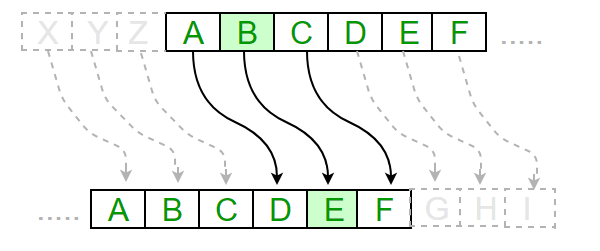
\includegraphics[scale=0.3]{images/caesar_cipher.png}
  \end{figure}

  Example: $``I LOVE CRYPTOGRAPHY'' \rightarrow
  ``L ORYH FUBSWRJUDSKB''$

  \pause

  \vspace{\baselineskip}
  Symmetric(-Key) Cryptography
}

\frame{
  \frametitle{Cryptography}
  \framesubtitle{Vocabulary}

  Symmetric Cryptography diagram: \\~\

  $$ plain text \xrightarrow[key]{encryption}
  cipher \xrightarrow[key]{decryption} plain text $$
}

\frame{
  \frametitle{Cryptography}
  \framesubtitle{Symmetric cryptosystem examples}

  \begin{itemize}
  \item Caesar cipher
  \item Data Encryption Standard (DES) (1975)
  \item Advanced Encryption Standard (AES) (1998)
  \end{itemize}
}


\frame{
  \frametitle{Cryptography}
  \framesubtitle{Issues with symmetric cryptography}

  \begin{itemize}
  \item Sharing key with other parties
  \item Different key for every party
  \end{itemize}

  $\rightarrow$ Public Key cryptography
}

\frame{
  \frametitle{Cryptography}
  \framesubtitle{Public key cryptography}

  One way functions
  \pause

  In $\mathbb{Z}/100\mathbb{Z}$ (numbers modulo 100)

  $$ f : n \mapsto n^2 $$

  $f(41) = 41^2 = 1681 = 81 \pmod{100}$

}

\frame{
  \frametitle{Cryptography}
  \framesubtitle{Public key cryptography}

  RSA (Rivest--Shamir--Adleman 1977)
  \begin{itemize}
  \item Public Key: modulo $n$, number $e$
  \item Private Key: number $d$
  \end{itemize}
  Such as for any $x$, number modulo $n$:
  $$ x^{e.d} = x \pmod{n} $$

  \pause

  Encryption: $ p \mapsto p^e $ ;
  Decryption: $ c \mapsto c^d $
}

\frame{
  \frametitle{Cryptography}
  \framesubtitle{Issues with public key cryptography}

  Slow, can only encrypt little data
  (by design -- one-way functions)

  Anybody can encrypt data: no more sender validation

  \vspace{\baselineskip}
  $\rightarrow$ Digital Signatures
}

\frame{
  \frametitle{Cryptography}
  \framesubtitle{Signing / Validating}

  Use Public Key Cryptography to sign: but ``encrypt'' with private
  key.

  \pause

  \begin{itemize}
  \item Public Key: modulo $n$, number $e$
  \item Private Key: number $d$
  \end{itemize}
  Such as for any $x$, number modulo $n$:
  $$ x^{e.d} = x \pmod{n} $$

  Encryption: $ p \mapsto p^e $ ;
  Decryption: $ c \mapsto c^d $

  \pause

  Signing: $ p \mapsto p^d $ ;
  Validation: $ s \mapsto s^e $
}

\frame{
  \frametitle{Cryptography}
  \framesubtitle{Issues with signatures}

  Signing proves that you own the Key Pair.

  \pause
  \vspace{\baselineskip}

  But how do you prove who you actually are?

  \pause
  \vspace{\baselineskip}

  $\rightarrow$ Certificates
}


\frame{
  \frametitle{Cryptography}

  Questions?
}

\section{Certificates}
\frame{
  \frametitle{Certificates}
  \framesubtitle{Examples}

  \begin{itemize}
  \item birth certificate
  \item marriage certificate
  \item state ID
  \item driver's license
  \item international passport
  \end{itemize}

  What do they have in common?
}

\frame{
  \frametitle{ID cards}
  \framesubtitle{why do we use them?}

  Why do we have IDs?

  \pause

  Proof for information

  \pause

  The 3 main categories on an ID card?

  \pause

  \begin{itemize}
  \item Proof that it belongs to a certain entity \& method for
    anybody to validate that
  \item Proof that it was emitted by a trusted authority
  \item Data the entity wants certified
  \end{itemize}

  \pause

  Authorities in place:
  \begin{itemize}
  \item State government: Certificate Authority (CA)
  \item DMV: Registration Authority (RA)
  \item TSA agent with ultraviolet light: Validation Authority (VA)
  \end{itemize}
}

\frame{
  \frametitle{Digital Certificates}
  \framesubtitle{identity}

  electronic-IDs for software \pause :

  \begin{itemize}
  \item X.509
    \begin{itemize}
    \item Name / URL
    \item trusted signature
    \item public key
    \end{itemize}
  \end{itemize}

  Formalized concepts of CA and RA.
}

\frame{
  \frametitle{Certificates}

  Questions?
}

\section{Communicating safely using cryptography}
\frame{
  \frametitle{Using cryptography to communicate safely}

  \begin{itemize}
  \item Encrypt data so that it can only be read by entity with decoding key
  \item Making sure that the right entity has the decoding key
  \end{itemize}

  \pause
  \begin{itemize}
  \item Encrypt AES key with RSA
  \item Sign RSA public keys / owner by trusted party \pause : certificates
  \end{itemize}
}

\subsection{SSL / TLS}
\frame{
  \frametitle{SSL / TLS}
  \framesubtitle{TLS - Transport Layer Security}
  \begin{itemize}
  \item Cryptographic protocol for safe communication over computer network
    \pause
  \item Previously: SSL - Secure Sockets Layer (1994)
    \pause
  \item TLS 1.0 (1999)
  \item Now TLS 1.3 (2018)
  \end{itemize}
}


\frame{
  \frametitle{SSL / TLS}
  \framesubtitle{TLS handshake (simplified)}

  \pause
  \begin{enumerate}
  \item Client makes $https$ call to server: initiates TLS handshake
  \item Server sends its $x509$ certificate
  \item Client validates certificate signature against CA
  \item Client validates certificate hostname and gets public key $p$
  \item Client generates random string to be symetric private key $k$
  \item Client encrypt $k$ with server's public key $p$, and sends it to the server
  \item Server decrypts encoded key with its private key
  \end{enumerate}

  \pause
  End of handshake:
  \begin{itemize}
  \item client validated identity of server
  \item both parties have secure secret key for encrypted private communication
  \end{itemize}

  \pause
  Server and client will now communicate by encoding and decoding any data sent
  over the wire with their private key, using a symetric algorithm like AES.
}

\frame{
  \frametitle{How does TLS work?}
  \framesubtitle{Why is it secure?}

  \begin{itemize}
  \item encrypts data
  \item makes sure the right entity can decrypt
  \end{itemize}
}

\frame{
  \frametitle{TLS}

  Questions?
}

\frame{
  \frametitle{TLS}
  \framesubtitle{What is --skip-ssl-validation?}

  Or in the browser ``This page in not secure...''
  \pause

  Not encrypting data? \pause Yes it is.
  Not validating identity: self-signed certificate.
}

\frame{
  \frametitle{mTLS}
  \framesubtitle{mutual TLS}

  \begin{itemize}
  \item With TLS, client validates identity of server. Client doesn't authenticate.
  \item Most websites use username/password for client authentication.
  \item mTLS can be done with username/password: we'll look at certificate based mTLS
  \end{itemize}

  \pause
  Not MTLS
}

\frame{
  \frametitle{mTLS}
  \framesubtitle{mutual TLS}

  \begin{enumerate}
  \item server sends its certificate to client
  \item client validates certificate signature and hostname
  \item client sends its certificate to server
  \item server validates certificate signature
  \item server generates random key to use as private symmetric key and sends
    to client
  \end{enumerate}

  \pause

  Both entities validated that the other party is trustworthy
}

\frame{
  \frametitle{mTLS}
  \framesubtitle{TLS termination}

  \begin{itemize}
  \item TLS termination proxy
  \item TLS forward proxy
  \end{itemize}
  \pause
  CF does mostly TLS forward proxy, calls it TLS termination proxy
}


\section{PKI}
\subsection{What is a public key infrastructure?}
\frame{
  \frametitle{PKI}

  A PKI consists of:
  \begin{itemize}
  \item A certificate authority (CA)
  \item A registration authority (RA)
  \item A central directory (for key storage)
  \item A certificate management system (e.g. who can access the stored keys)
  \item A certificate policy (stating the PKI's requirements concerning its procedures.
    Its purpose is to allow outsiders to analyze the PKI's trustworthiness.)
  \end{itemize}
}

\section{Tokens}
\frame{
  \frametitle{Tokens}
  \framesubtitle{Tokens in real life}

  An object that can be exchanged for something else.
  \pause
  \begin{itemize}
  \item Fair token \pause
  \item Money (cash, bank statement)
  \item Checks
  \end{itemize}

  \pause

  What do they have in common?

  \pause

  \begin{itemize}
  \item They can be exchanged for something of value,
    but have no other value
  \item Proof to the receiver that the token is legitimate
    (that is was created by a trusted issuer) \pause
  \item Difficult to replicate
  \end{itemize}

}

\section{Tokens}
\frame{
  \frametitle{Tokens}
  \framesubtitle{Digital Tokens}

  Cannot be made difficult to replicate.  Security has to come
  from something else: secrecy. \pause

  Two large categories for digital tokens:

  \begin{itemize}
  \item Opaque tokens
    (a sequence of bytes that the issuer knows about)
  \item Transparent tokens \pause
    \begin{itemize}
    \item JWT (JSON Web Token)
      \begin{itemize}
      \item payload
      \item signature
      \end{itemize}
    \end{itemize}
  \end{itemize}

  \pause

  \begin{tabular}{ccc}
    
\includegraphics[scale=0.03]{images/warning.jpg} &
    \raisebox{\totalheight}{Signature does not mean it's safe to share.} &
    
\includegraphics[scale=0.03]{images/warning.jpg} \\
  \end{tabular}
}

\section{OAuth}

\frame{
 \frametitle{OAuth}
 \framesubtitle{Example: login with Google}

 \begin{figure}
   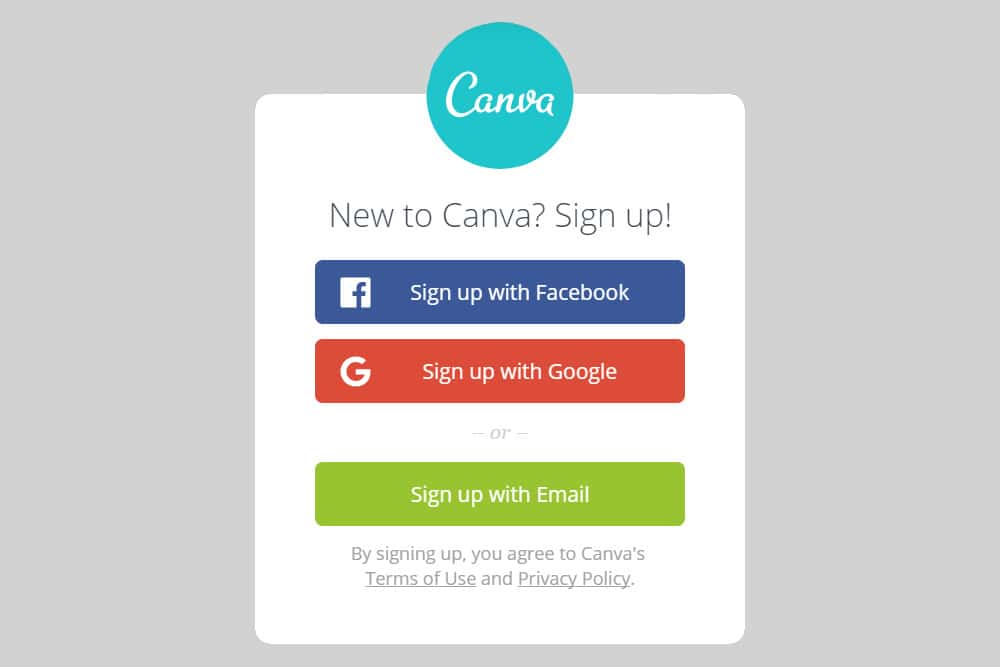
\includegraphics[scale=0.3]{images/login-with.jpg}
 \end{figure}
}

\frame{
 \frametitle{OAuth}
 \framesubtitle{Example: SSO}

 \begin{figure}
   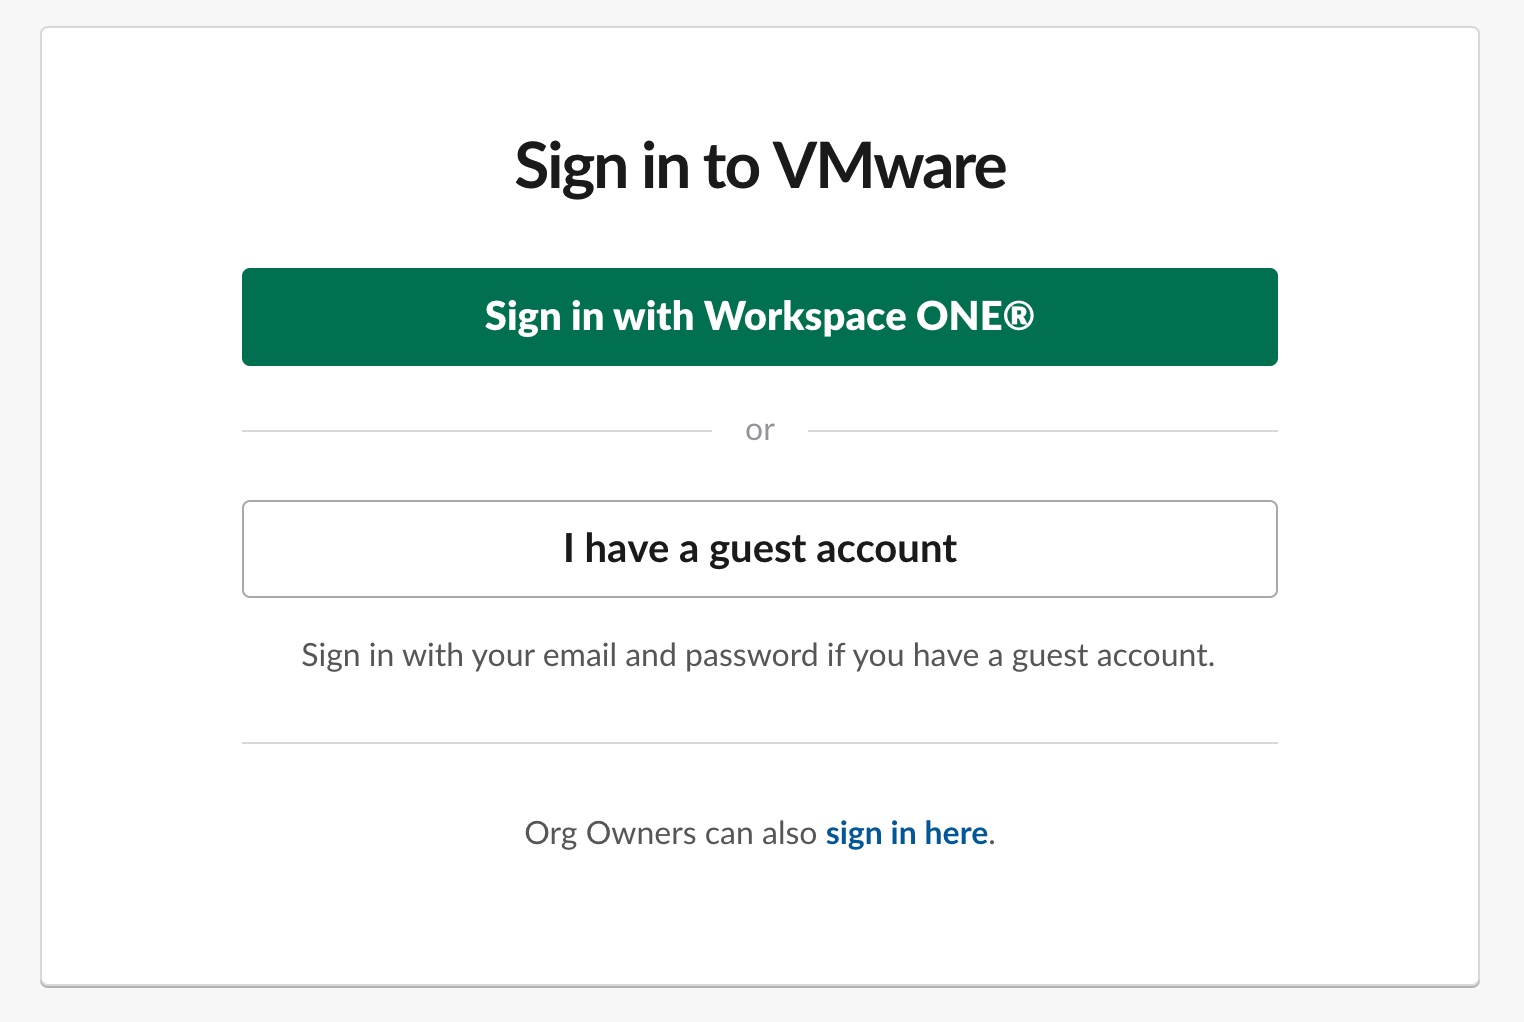
\includegraphics[scale=0.4]{images/slack.png}
 \end{figure}

}

\frame{
 \frametitle{OAuth}
 \framesubtitle{What is it?}

 To sign-up, you'll have to enter a lot of information (time
 consuming). OR, you can have the service contact Facebook or Google
 to get your name, email, profile picture, birth date etc. and the
 website will then create for you an account using this information. \\~\

 You are NOT really logging-in with Facebook. \\
 It's more like you're signing-up using your Facebook data.

}

\section{Extras}

\frame{
  \frametitle{Safe key exchange}
  \framesubtitle{Diffie Helmann}

  \begin{itemize}
  \item Issue with exchanging private keys with symmetric algorithm
    if private key gets lost
  \item Diffie Helmann algorithm
  \end{itemize}
}
\end{document}
